\chapter{Introduction}
\label{cha:intro}

% TODO: The first chapter contains a general introduction to the work. The goals are defined and the modus operandi is explained.

The mobile industry is without a doubt one of the most vibrant industries at the moment. It is characterized by rapid growth and intense competition which has led to fragmentation. 

This chapter presents an overview of the evolution in the mobile device landscape, explains the problem of fragmentation and how cross-platform tools (CPTs) can solve this problem.

\section{The mobile device landscape}

\subsection{Smartphones}

Mobile phones have been around since the nineties and before but the smartphone as we know it now has only been around since the (nearly simultaneous) introduction of the iPhone 3G and the HTC Dream in 2008. In the last five years, smartphone sales have grown tremendously. According to quarterly studies by Gartner\footnote{Gartner is an American firm, specialized in information technology research \cite{Gartner}.} \citeGartner, smartphone sales have grown 544\% since the second quarter of 2008 (see \fref{fig:smartphone-sales}). Smartphones are becoming ubiquitous and in some regions like the United States, smartphone penetration has already reached more than 50\% \cite{Nielsen:2012}. 

\begin{figure}[h!]
    \begin{center}
        \TODO{Update Graph} 
        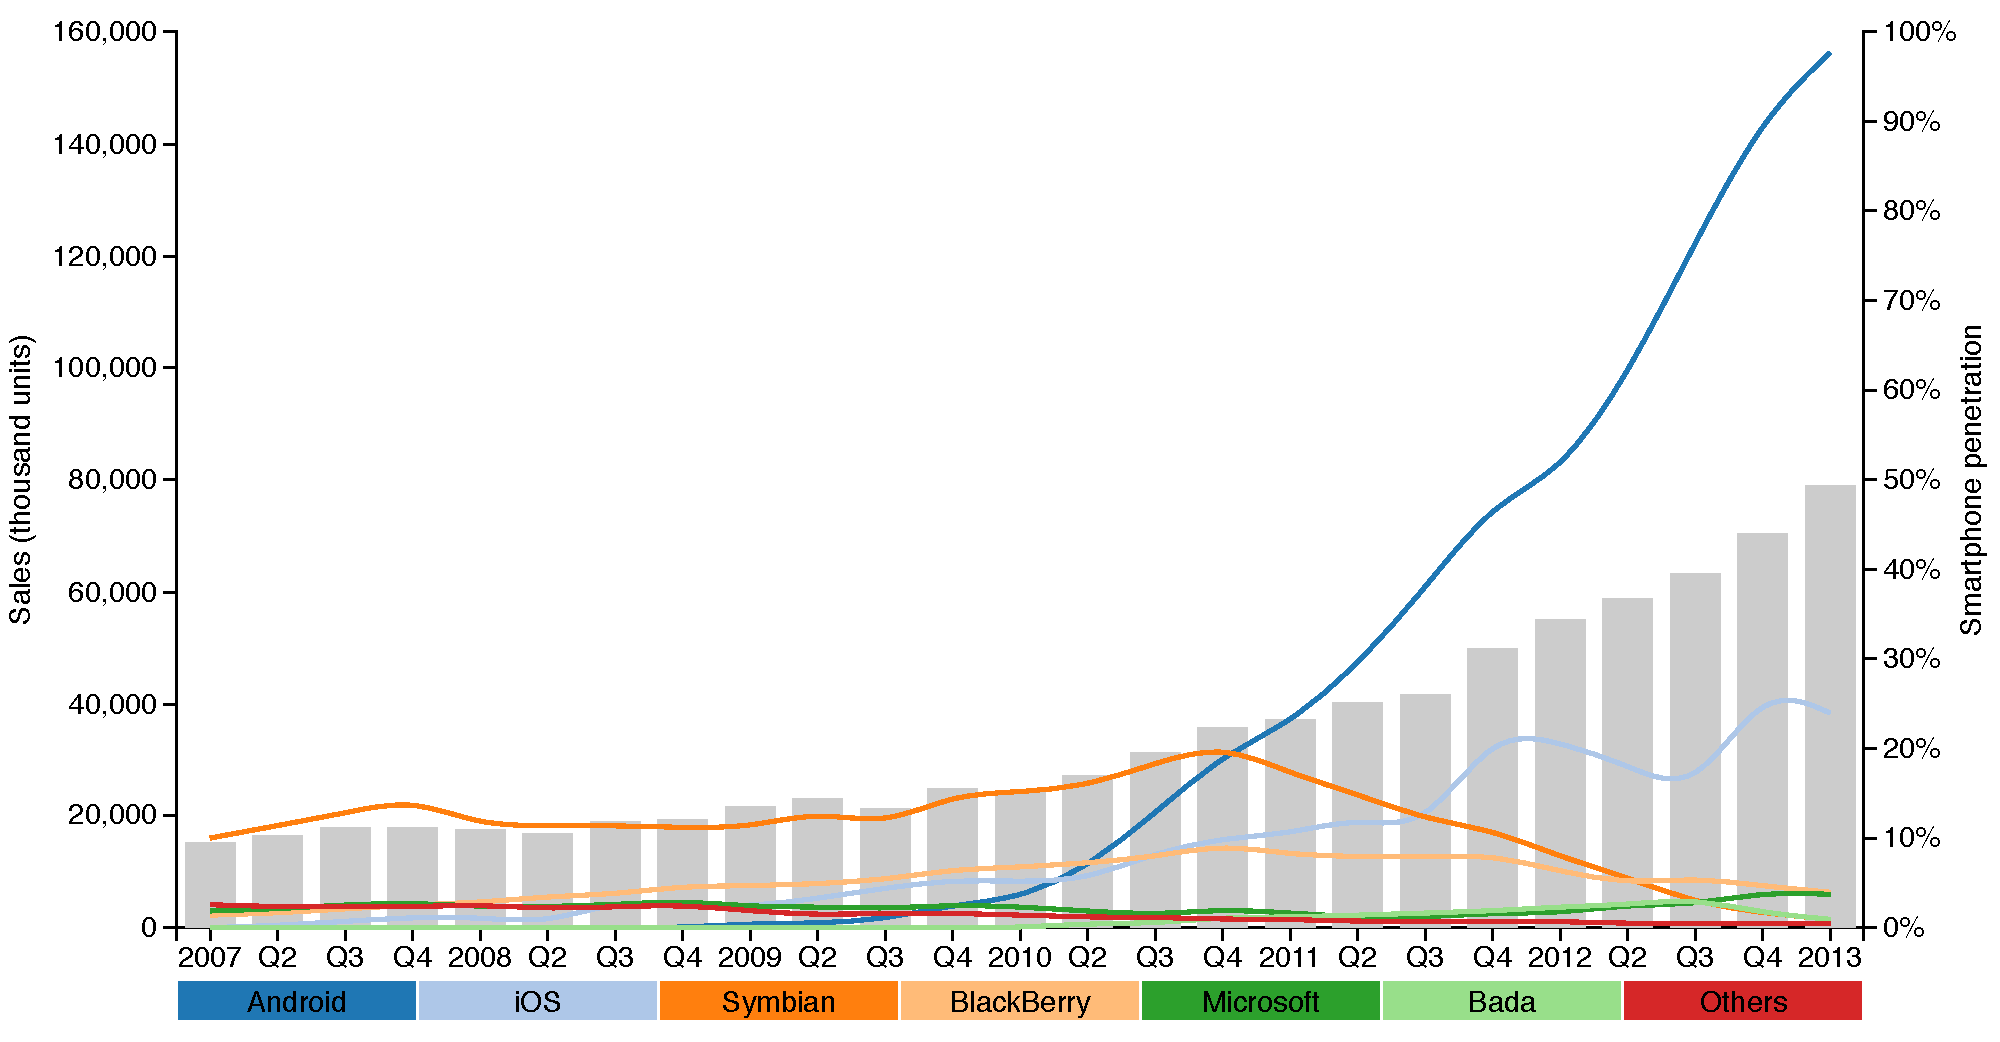
\includegraphics[width=\textwidth]{figs/smartphone_sales.pdf}
        	\caption{
        	    Growth of worldwide smartphone sales and smartphone penetration.\newline
        	    Source: Gartner \citeGartner
        	}
        	\label{fig:smartphone-sales}
    \end{center}
\end{figure}

\begin{figure}[h!]
    \begin{center}
        \TODO{Update Graph} 
        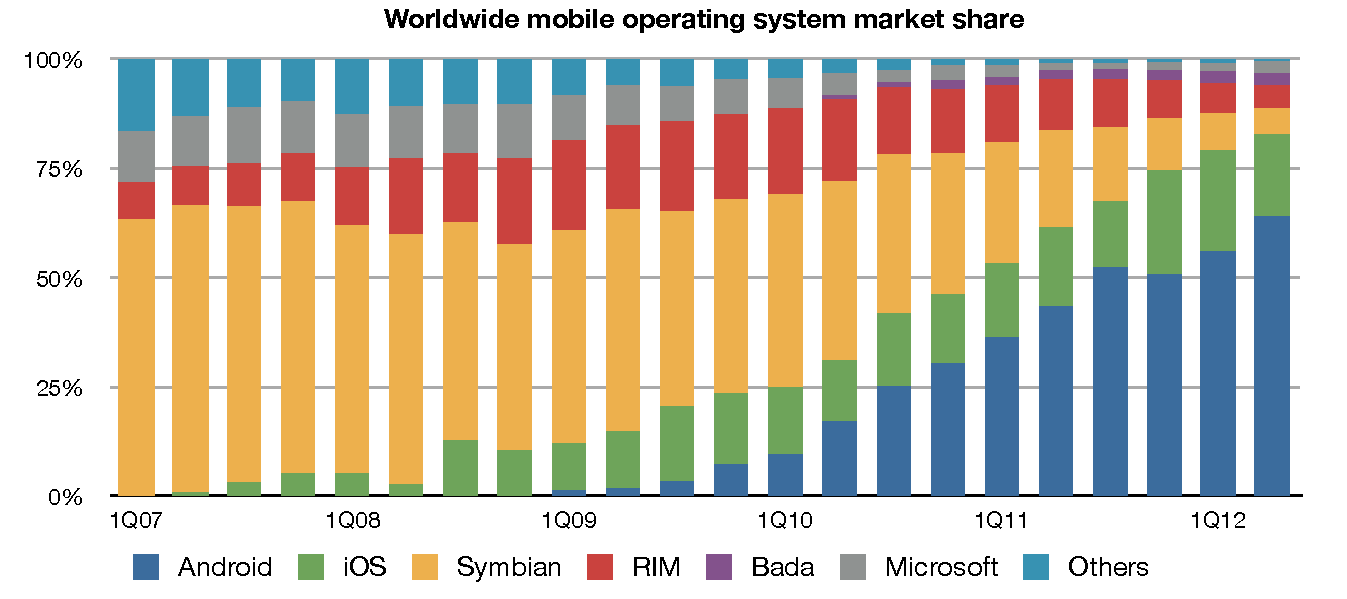
\includegraphics[width=\textwidth]{figs/smartphone_os.pdf}
        \caption{
            Growth of worldwide smartphone operating system market share.\newline 
            Source: Gartner \citeGartner
        	}
        \label{fig:smartphone-share}
    \end{center}
\end{figure}

Operating systems are heavily subjected to network effects, i.e. the value of a platform is proportional to the number of people using it. This makes it hard for new platforms to gain traction which is visible in \fref{fig:smartphone-sales} and \fref{fig:smartphone-share}. Android and iOS are currently the most popular platforms and other platforms are either in decline (like Symbian and Blackberry, formerly RIM) or have a hard time getting traction (like Windows Phone).

However, there is so single major platform. The IDC\footnote{International Data Corporation is another American market research firm, specializing in information technology, telecommunications and consumer technology.} even predicts that Windows Phone will gain a significant market share by 2016 and that 90\% of the worldwide smartphone market will then be covered by Android, iOS and Windows Phone \cite{IDC:phone}. Therefore it is very reasonable to assume that there will always be more than one major platform.

\subsection{Tablets}

A similar scenario is playing out in the tablet industry. According to other studies by both Gartner \citep{Gartner:11tab,Gartner:12tab} and the IDC \citep{IDC:tablet}, tablets will continue to gain popularity and sales will be mainly driven by iPads and Android tablets (see \fref{fig:tablet}).

\begin{figure}[h!]
    \begin{center}
        \TODO{Check whether new predictions are available} 
        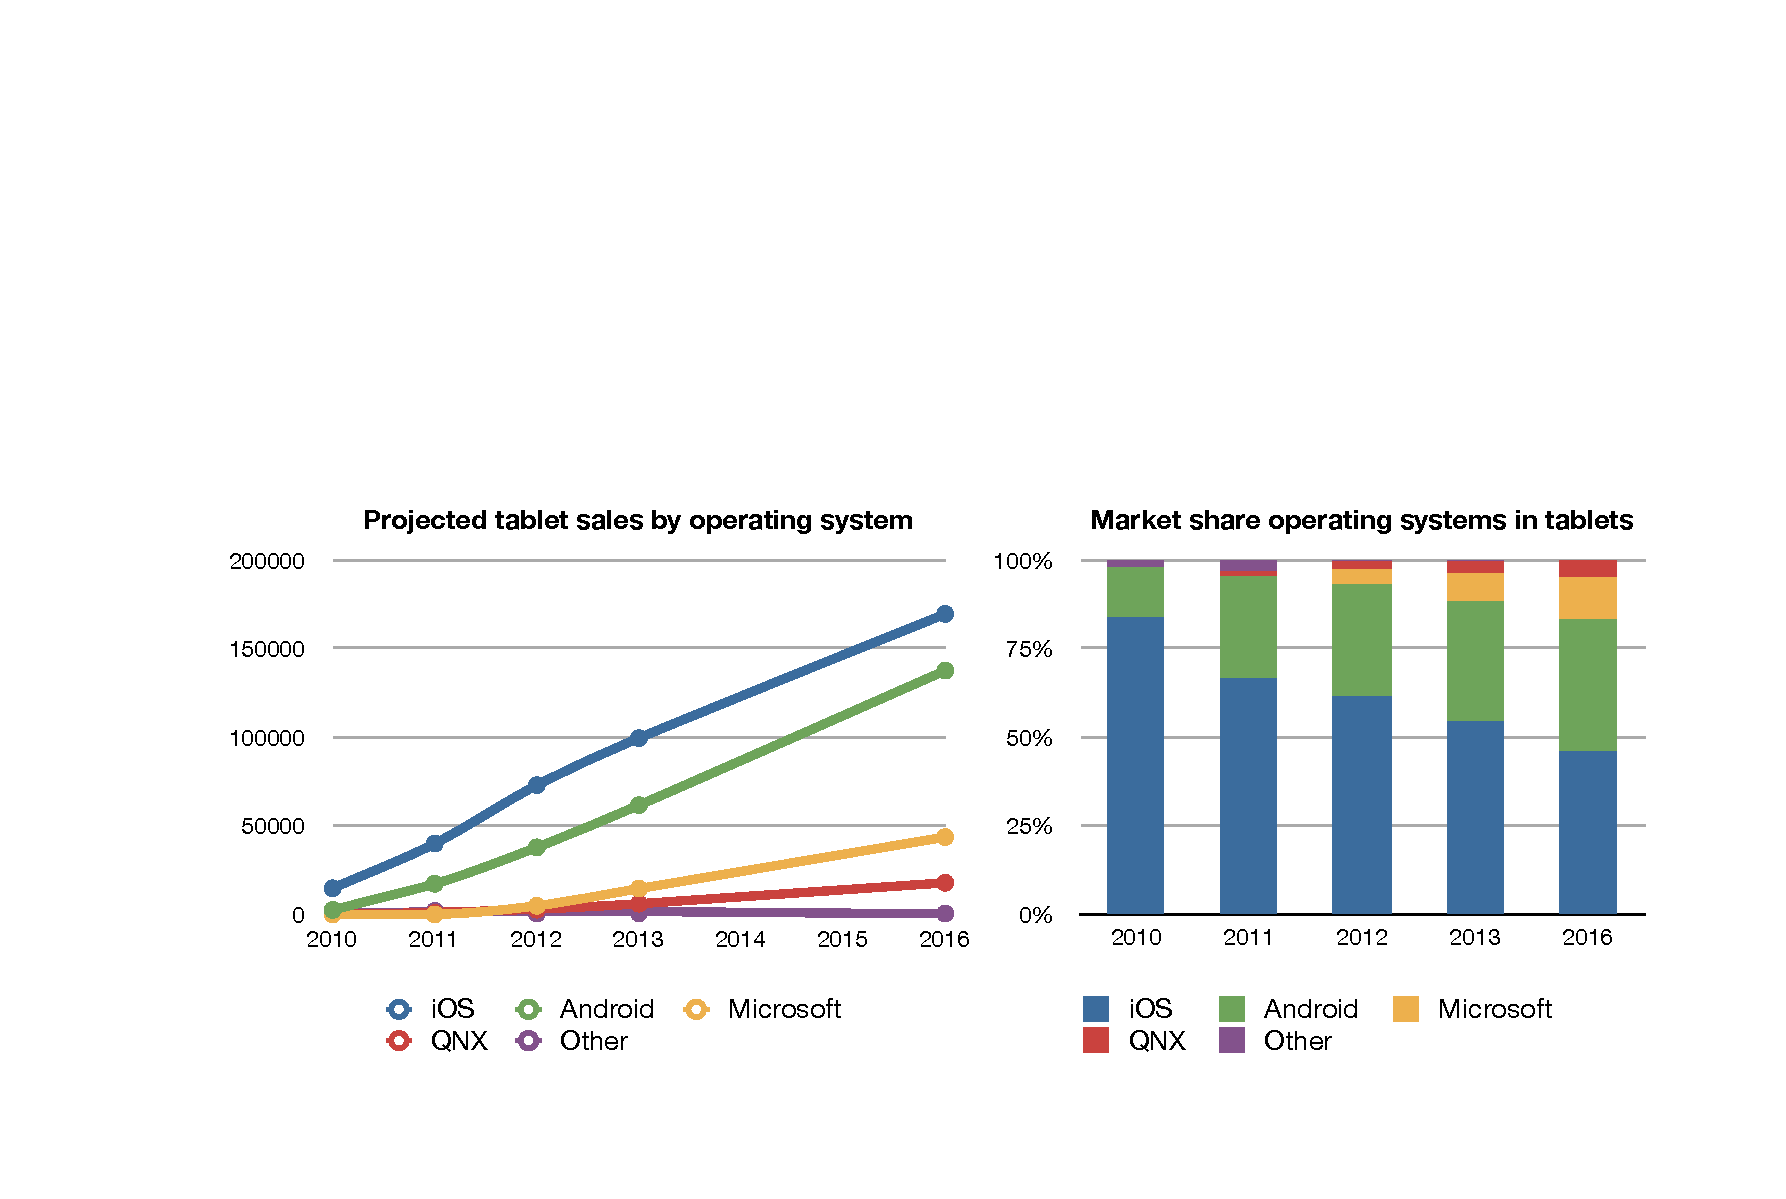
\includegraphics[width=\textwidth]{figs/tablet.pdf}
        \caption{
            Prediction of worldwide tablet sales and market share.\newline
            Source: Gartner \citeGartnerTab
        }
        \label{fig:tablet}
    \end{center}
\end{figure}

Even though both companies do not agree on which platform will serve the most devices, they both predict there will be at least three major platforms: iOS, Android and Windows. 

\section{The problem of fragmentation}

The competition among mobile device manufacturers has led to fragmentation on many levels. For consumers, carriers and manufacturers, fragmentation is usually a good thing. The more different devices there are, the easier it is for consumers to pick the device that fits their needs. 

For developers on the other hand, fragmentation is usually a bad thing. They will have to develop and test their applications on multiple devices to be able to guarantee the desired experience. This is expensive and time consuming.

Fragmentation is a multi-dimensional problem. From \fref{fig:smartphone-share} and \fref{fig:tablet} it is already clear that the operating system or platform is one obvious dimension; this is called platform fragmentation. Other dimensions include device configuration, runtime, user interface, etc.

The next subsections will discuss fragmentation issues within iOS and Android.

\subsection{Fragmentation within iOS}

Devices running iOS (commonly referred to as iDevices) are available in different shapes and sizes. Yet, there are only a limited number of (similar) device configurations in two form factors: iPhone (covering iPhone and iPod Touch devices) and iPad. Apple uses these form factors to distinguish three kinds of applications: iPhone apps (designed to run on iPhone form factor only), iPad apps (designed to run on iPad only) and universal apps (designed to run on both form factors). 

% TODO: describe runtime fragmentation
\TODO{describe runtime fragmentation}

Overall, Apple can manage fragmentation quite well and fragmentation is rather low within iOS.

\subsection{Fragmentation within Android}

Android is an open source platform, developed by Google. Manufacturers are allowed to tailor it for their devices and many of them have grabbed this opportunity to differentiate their products. On april 24 2013, the Google Play store officially supported 2827 device configurations, distributed across 59 manufacturers. The ability to alter the operating system has largely contributed to the success of Android.

There is however virtually no incentive for device manufacturers to maintain their Android flavours and as a result they do not often provide updates for their devices. This has led to the notorious runtime fragmentation among Android devices (see \fref{fig:runtime_fragmentation}).

\begin{figure}[h!]
    \begin{center}
        % TODO: runtime fragmentation evolution
        \TODO{It would be nice to have an overview of Android version adaption, maybe use the internet archive and http://developer.android.com/about/dashboards/index.html. Also mark introduction dates of version.}
        \label{fig:runtime_fragmentation}
        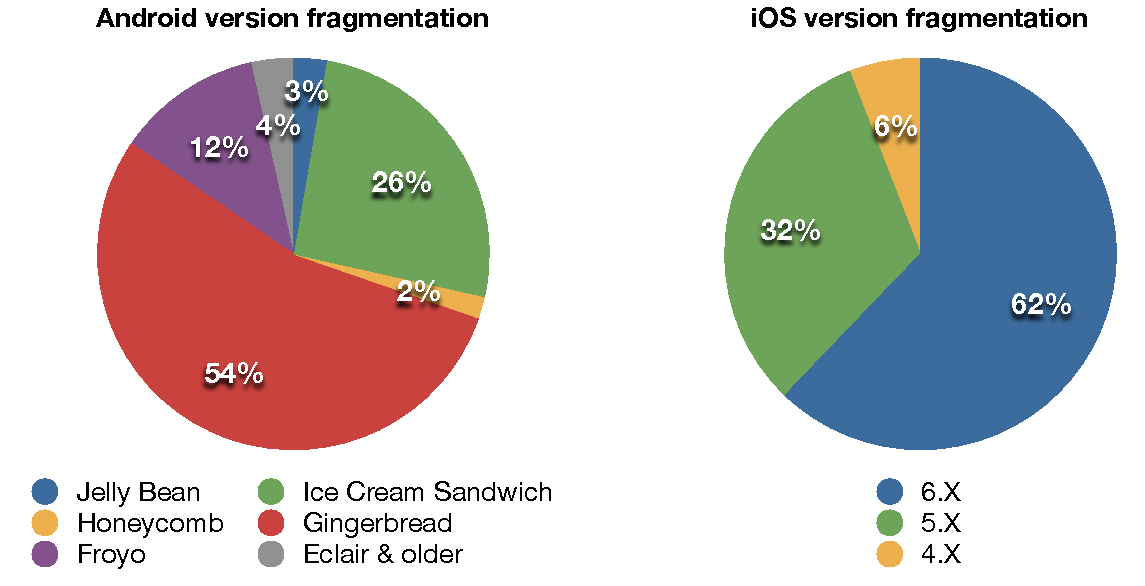
\includegraphics[width=0.8\textwidth]{figs/os_distribution.pdf}
        \caption{
            Runtime fragmentation for Android (data collected by Google during a 14-day period ending on November 1, 2012) \citep{android_distribution} and iOS (based on the statistics of developer David Smith) \citep{ios_distribution}.
        }
    \end{center}
\end{figure}

These flavours also contribute to user interface fragmentation because manufacturers ship their devices with a custom user interface to differentiate their product.

Because of the sheer number of Android devices, there is also a large  number of CPUs, screen sizes, display resolutions, pixel density configurations and many more. All these differences contribute to device fragmentation. 

Long story short, the Android platform is characterized by fragmentation in all dimensions.

\section{Cross-Platform Tools to the rescue}

In the current economy, information is a company's most valuable asset and the rate at which information exchange takes place increases every day. Mobile Internet-enabled devices are a valuable resource for this purpose and, as a consequence, many companies want mobile applications for their businesses.

However, in an ever-changing and unpredictable industry like the mobile industry, it is very unwise to target a single platform. This could eventually lead to lock-in situations which companies try to avoid at all costs. Consequently, they will ask for a cross-platform solution. 

Cross-Platform Tools (CPTs) can help solving this problem. They reduce entry barriers (access to new platforms) and exit barriers (lock-in) by allowing developers to create cross-platform applications from a single codebase \cite{VMCPT:2012}. 

Cross-Platform Tools try to solve three major problems \cite{VMCPT:2012}: 

\begin{enumerate}
    \item \textbf{Fragmentation} The fragmentation issues described above are a pain for every developer. They need to test their applications on a large number of devices in order to be able to guarantee the desired user experience. A CPT can help to identify platform quirks and can provide workarounds. 
    \item \textbf{Access to new platforms and screens} Targeting a new platform or screen (for instance, television sets or car consoles) is often hard. Developers need to learn yet another SDK and/or programming language in order to deliver applications for the platform or screen. Using a CPT can drastically reduce the effort needed to target a new platform or screen.
    \item \textbf{Development inefficiency} Maintaining codebases for multiple platforms is a difficult task. When using a CPT, all code is contained within a single codebase and no time is lost while synchronizing features and other maintenance tasks across codebases. 
\end{enumerate}

% TODO: finish Chapter
\TODO{Finish chapter, which can be read where + define scope, make boundaries}


